
En la siguiente aparatado intentamos validar dos hipótesis: que el modelo generado realmente puede ser identificado como un hablante extranjero de habla inglesa y al mismo tiempo que este posee un grado de inteligibilidad aceptable.

Para eso se condujo una encuesta perceptual donde a cada participante se le presentó una oración sintetizada con distintos grados de mezcla de español e ingles y se le pidió que la transcribiera y que intentara identificar la nacionalidad del hablante. Para evitar que el participante pudiera deducir las palabras a partir de las palabras vecinas, las mismas son generadas de manera semánticamente impredecible. Esto significa que a partir de una lista de sustantivos, adjetivos, determinantes y verbos se generan oraciones de manera aleatoria con la estructura:

$$\textnormal{\textit{Determinante Adjetivo Sustantivo Verbo Determinante Sustantivo}}$$

Luego, para asegurarnos de estar cubriendo todos los posibles fonos del castellano, las oraciones son modificadas para ser fonéticamente balanceadas. Esto querrá decir que incluimos entre cinco y diez veces cada fono perteneciente a una consonante (presente en el repertorio del castellano) y al menos veinte veces cada fono perteneciente a una vocal.

Los oraciones finalmente generadas fueron:

\begin{itemize}
\item Oración 1: Mi montaña aguileña recorrió la esquina
\item Oración 2: Aquel fuerte vidrio prefirió aquel botón
\item Oración 3: Este enjoyado juez comprará nuestro corchete
\item Oración 4: Tu estrecho posavasos gritó la fechoría
\item Oración 5: Nuestro nublado tigre concluyó a este chupetín
\item Oración 6: Su profundo riñón apoyó a Julio
\item Oración 7: El frío churrasco oyó lo de Polonia
\item Oración 8: Las acongojadas cotorras sonrieron a mi círculo
\item Oración 9: Ese gruñón perro prometió a esos cuñados
\item Oración 10: El nudillo Argentino perdió su vaso
\end{itemize}

Para cada uno de estos diez oraciones se varió el nivel de mezcla entre $30\%$ de ingles, $70\%$ castellano hasta $70\%$ de ingles, $30\%$ de castellano, $10\%$ cada vez. De esta manera, para cada oración habrá 5 mezclas diferentes, lo que hace un total de $50$ audios sintetizados diferentes.

La encuesta se realiza a través de internet, con el mismo set de instrucciones para todos los participantes y pidiendo como requerimiento la utilización de auriculares. Cada participante podía contestar un máximo $5$ veces (otorgándoles siempre audios distintos).

El objetivo de la misma es conseguir para cada uno de los $50$ audios sintetizados, $5$ respuestas, momento en el cual se cierra la posibilidad de contestar.

La misma se lleva a cavo desde el $18$ de octubre de $2017$ hasta el primero de diciembre del mismo año, tiempo durante el cual fue publicada en distintas redes sociales y listas de emails de la facultad.

Con el objetivo de no influir en las respuestas de los participantes, se procuró darles la información mínima indispensable para completar la encuesta. Por este motivo, en ningún momento de la encuesta se especifica el objetivo del estudio.

Con la intención de estandarizar los resultados, fue requisito obligatorio utilizar auriculares para la encuesta. También se le pidió a cada participante que la realizara en un lugar silencioso y tranquilo.

\section{Interfaz}

En este apartado se presenta la interfaz utilizada para realizar la encuesta junto con las decisiones de diseño más relevantes. 

En la figura \ref{personalData} se presenta la pagina principal en la que todos los participantes fueron recibidos.

\begin{figure}[htp]
\begin{center}
\fbox{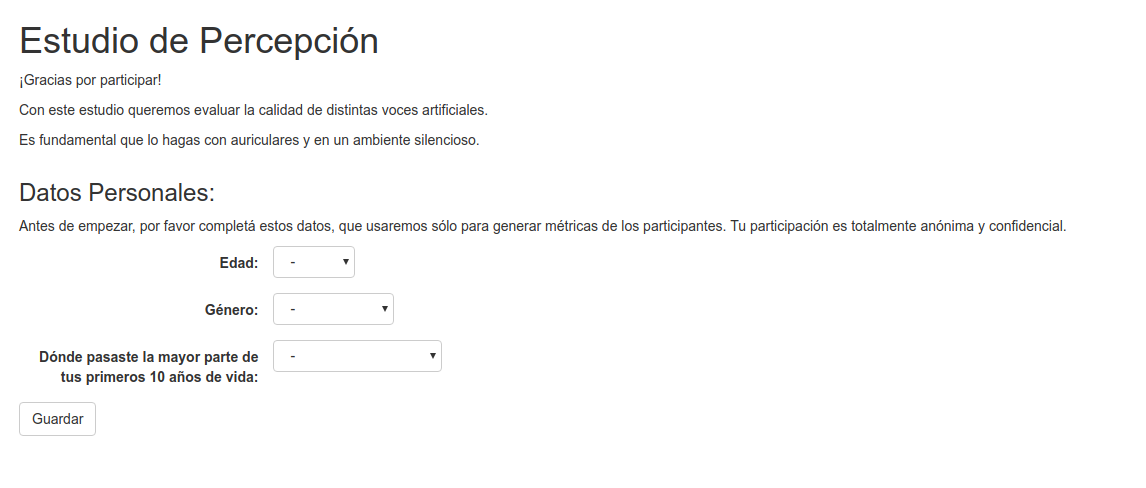
\includegraphics[scale=0.6]{estudio_online/estudio1.png}}
\end{center}
\caption{Datos Personales}
\label{personalData}
\end{figure}

A fin de conocer de manera general la demografía encuestada, a cada participante se le pidió que indique el rango correspondiente a su edad, yendo desde $18$ a $25$, $26$ a $35$, y así de diez en diez.

Se les pidió, además, que indicara su genero: masculino, femenino, otro, no contesta y la provincia donde pasó sus primeros diez años de vida. Consideramos que estos datos son importantes para el estudio ya que dependiendo de ellos los resultados variarán indefectiblemente, la transcripción que obtendremos de un participante de $50$ años de capital federal será distinta a la de alguien de $18$ años de Córdoba. El diferente uso de los alofonos, modismos y variantes prosódicas y capacidades auditivas jugarán un papel importante en la interpretación de la oración y la apreciación del origen del hablante.

Una vez que completados estos datos, se le presenta otra vista con las instrucciones especificas para completar la encuesta (figura \ref{instrucciones}).

\begin{figure}
\begin{center}
\fbox{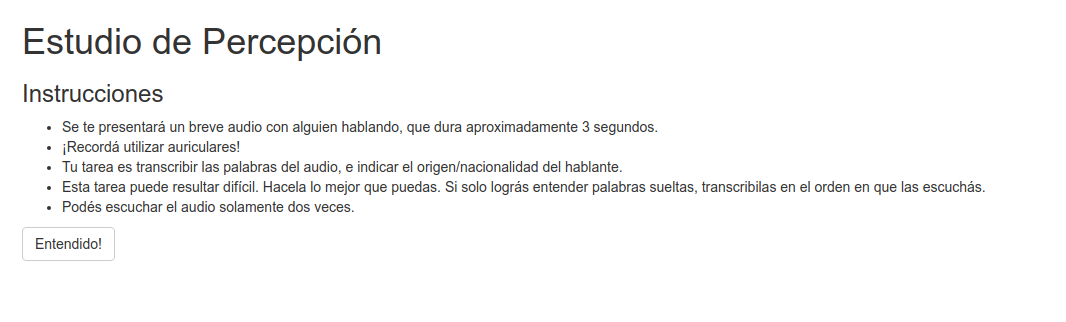
\includegraphics[scale=0.6]{estudio_online/estudio2.png}}
\end{center}
\caption{Instrucciones}
\label{instrucciones}
\end{figure}

Una vez presionado el botón de ``entendido!'' se les presentaba un audio, que podían escuchar un máximo de $2$ veces, una caja de texto libre donde plasmar la transcripción del mismo y una caja de texto libre donde podían escribir la nacionalidad correspondiente a la voz (figura \ref{transcripcion})

\begin{figure}
\begin{center}
\fbox{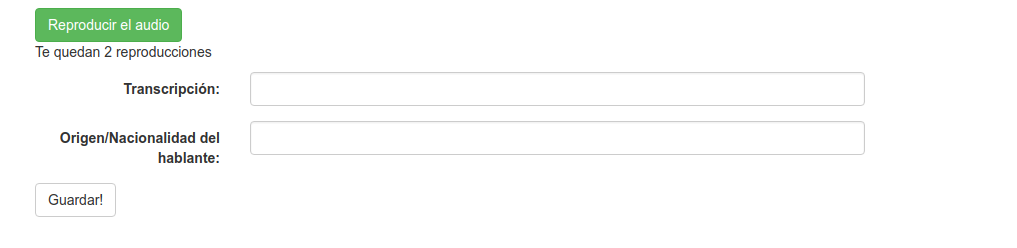
\includegraphics[scale=0.6]{estudio_online/estudio3.png}}
\end{center}
\caption{Transcripción}
\label{transcripcion}
\end{figure}

Una vez que la respuesta es guardada, se le preguntaba si quiere continuar transcribiendo otro audio, o de caso de haber contestado cinco veces, se le presentaba un mensaje donde se le indicaba que ya podía cerrar la encuesta (figura \ref{continuar}).

\begin{figure}
\begin{center}
\fbox{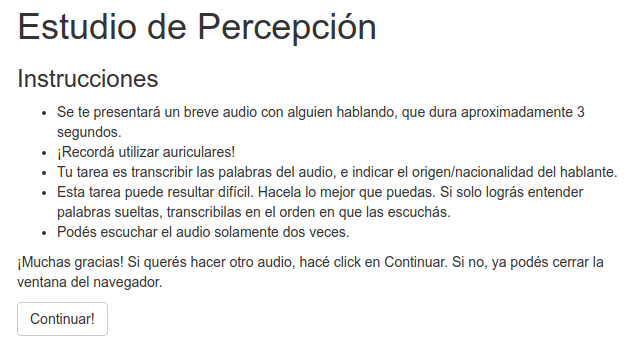
\includegraphics[scale=0.6]{estudio_online/estudio4.png}}
\end{center}
\caption{Dialogo Final}
\label{continuar}
\end{figure}